\chapter{Background}
\label{cha:background}

In this thesis, we will analyze in detail the behavior of an LLM as an agent within
a controlled environment.

Before presenting all the work carried out in detail, this chapter aims to
provide a comprehensive explanation of all the theoretical foundations necessary
to understand the steps presented in the following chapters. Starting from a brief
introduction of Artificial Intelligence just to define the boundaries in which we
are working, we will move to the core concepts. In particular, we want to
highlight what an LLM is and how it works, with a special focus on the Attention
mechanism and how the uncertainty of an LLM can be calculated. This will serve
as a basis for correctly interpreting the results analyzed in Section
\ref{cha:results_discussion}.

There will also be a broader discussion on agents in a strict sense and "LLM agents"
to better show the difference between our implementation and what is currently
being discussed over the media.

To better define the context of this thesis, we will examine the main alternative
approaches to solving a logistical problem currently studied in the literature.

\section{Artificial Intelligence}
\label{sec:artificial_intelligence}

Right now in the media, AI is being used as a synonym for Large Language Models.
However, AI is a broader concept that includes many techniques and methodologies.

\#\# Summary of different kind of AI ending with Generative Models end with NLP
history

\section{Large Language Models - LLMs}
\label{sec:large_language_models_llms}

\#\# LLMs are generative models released with the paper "Attention is All You
Need"

\subsection{LLMs' Uncertainty}
\label{sub:llms_uncertainty}

Understanding the uncertainty of an LLM is crucial to correctly interpret the text
it generates. If we ask for a yes/no question, it would make a different impact on
us reading "Yes" or "Yes - Uncertainty 49\%". Moreover, this would let us get
some kind of explainability behind these complex and opaque systems.

\#\# cite Hallucinations

\section{Agents}
\label{sec:agents}

% \begin{figure}[h!]
%   \label{fig:agent_scheme}
%   \centering
%   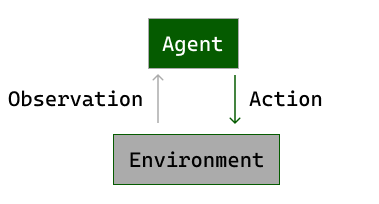
\includegraphics[width=.3333\textwidth]{images/Agent_Scheme.png}
%   \caption{Agent Scheme}
%   { Source: redesign of a scheme in \cite{wooldridge2002multiagent}}
% \end{figure}

As widely explained in the book ``An Introduction to Multiagent Systems" \cite{wooldridge2002multiagent},
we can summarize the definition of an agent as an autonomous entity that
perceives its environment through sensors and acts upon it through effectors, making
decisions based on its perceptions and objectives in order to achieve specific goals.

This definition highlights several key aspects of agents:
\begin{itemize}
  \item Autonomy: Agents operate without direct human intervention, controlling their
    own actions.

  \item Perception and Action: They interact with the environment via sensors (perception)
    and effectors (action execution).

  \item Decision-making: Agents select actions based on their internal model, goals,
    and the state of the environment.

  \item Non-determinism and Adaptability: Since environments are generally non-deterministic,
    agents must be prepared for uncertainty and potential failures in action execution.

  \item Preconditions and Constraints: Actions are subject to certain conditions
    that must be met for successful execution.
\end{itemize}

Thus, an agent's fundamental challenge is deciding which actions to perform in
order to best satisfy its objectives, given the constraints and uncertainties of
its environment.

\begin{figure}[h!]
  \centering
  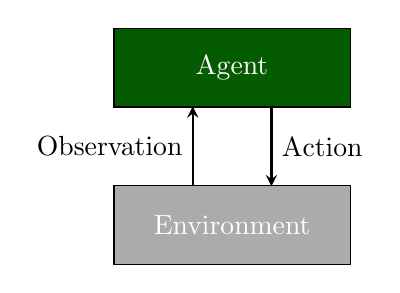
\begin{tikzpicture}[
    node distance=2cm, % Distance between nodes
  ]
    \node[
      rectangle,
      minimum width=3cm,
      minimum height=1cm,
      text centered,
      draw=black,
      fill={rgb,255:red,5; green,91; blue,0},
      text=white
    ] (agent) {Agent};
    \node[
      rectangle,
      minimum width=3cm,
      minimum height=1cm,
      text centered,
      draw=black,
      below of=agent,
      fill={rgb,255:red,171; green,171; blue,171},
      text=white
    ] (env) {Environment};

    % First arrow (Action) slightly shifted right
    \draw[thick, ->, >=stealth]
      (agent.south)
      ++(0.5,0) -- ++(0,-1)
      node[midway, right] {Action};

    % Second arrow (Observation) slightly shifted left
    \draw[thick, ->, >=stealth]
      (env.north)
      ++(-0.5,0) -- ++(0,1)
      node[midway, left] {Observation};
  \end{tikzpicture}
  \caption{Agent Design Scheme}
  { Source: redesign of a scheme in \cite{wooldridge2002multiagent}} \label{fig:agent_scheme}
\end{figure}

As shown in Figure \ref{fig:agent_scheme}, an agent is some entity that perceives
the environment and reacts to it. The environment can be anything from a simple
thermostat to a complex system like a self-driving car. The idea is that the agent
is able to react to a change in the environment and take actions to achieve its goals.

We will analyze in detail the prompts and the choices in the Chapter \ref{cha:data_collection}
Section \ref{sec:prompts}, but to give an some kind of help to align with the
definition above, we can map some of its concept to what this thesis will analyze:
\begin{itemize}
  \item Perception and Action: what the server sends about the current state of
    the environment can be seen as the perception of the agent, while the action
    it can take will be given in the prompt in a specific way.

  \item Decision-making: the decision-making process will be the generation of
    the text by the LLM, weighted by the uncertainty.

  \item Non-determinism and Adaptability: to emulate the non-determinism of the
    environment, the state received by the server will be used "raw" in the prompt,
    without any hard processing or parsing.

  \item Preconditions and Constraints: living in a "limited" map with a fixed
    number of cells, is itself a constraint the agent must consider.
\end{itemize}

\subsection{BDI Architecture}
\label{sub:bdi_architecture}

The Belief-Desire-Intention (BDI) architecture is a widely adopted framework in
artificial intelligence (AI) for modeling rational agents. It was formally developed
by Rao and Georgeff in 1995 \cite{bdi-icmas95} and has been implemented in several
architectures, including PRS (1987), dMARS (1998), JAM (1999), Jack (2001), and
JADEX (2005). BDI provides a structured approach to practical reasoning,
allowing agents to function effectively in dynamic and unpredictable
environments.

\subsubsection{Core Components of BDI}
BDI agents operate based on three key components:
\begin{itemize}
  \item Belief: Represents the agent’s knowledge about the world, including past
    events and observations. Given the agent's local perception and limited
    computational resources, beliefs act as cached, imperfect information rather
    than absolute knowledge

  \item Desire (Goals): Defines the agent’s objectives or preferred end states, such
    as "desiring to graduate." Desires help in justifying why an agent takes
    specific actions and enable reasoning about goal interactions, particularly in
    failure recovery scenarios

  \item Intention: Represents the commitments of an agent toward achieving
    specific goals through selected plans. Intentions provide structure by ensuring
    persistence and internal consistency, allowing for incremental planning and
    adaptation in real-time. They also serve as a means of coordinating multiple
    agents in distributed systems.
\end{itemize}

BDI has been extensively used in fields like robotics, automated planning, and
multi-agent systems. For instance, JADEX is a popular Java-based BDI framework
used in simulations and decision-making applications.

\section{State of the Art}
\label{sec:state_of_the_art}

A logistic problem is a fundamental challenge in the field of Artificial Intelligence
(AI), encompassing tasks such as route optimization, supply chain management,
and delivery scheduling. These problems arise in various domains, including
transportation, e-commerce, and manufacturing, where efficient resource allocation
and decision-making are critical. Given the complexity of modern logistics, AI has
emerged as a powerful tool for finding optimal or near-optimal solutions.

Several AI-based approaches can be used to address logistic problems.
Traditional operations research techniques, such as linear programming and heuristics,
have been widely employed. However, with the increasing availability of data and
computational power, machine learning (ML) and deep learning methods have become
more prevalent. These methods can predict demand, optimize routes dynamically,
and enhance decision-making under uncertainty. Additionally, reinforcement
learning (RL) has gained attention for its ability to learn optimal strategies
through trial and error, particularly in dynamic and unpredictable environments.

In the recent years with the explosion of Large Language Models (LLMs), many
researchers started to apply them to different fields, including planning and logistics.

% \begin{quotation}
%   This is a longer blockquote that may span multiple paragraphs. It is indented
%   on both sides.
% \end{quotation}

\subsection{PDDL Based Solutions}
\begin{blockquote}
  \textbf{Planning Domain Definition Language} (PDDL) is a human-readable format
  for problems in automated planning that gives a description of the possible
  states of the world, a description of the set of possible actions, a specific
  initial state of the world, and a specific set of desired goals.

  \emph{Source: Wikipedia\footnotemark}
\end{blockquote}
\footnotetext{\url{https://en.wikipedia.org/wiki/Planning_Domain_Definition_Language}}

The fundamental distinction between a PDDL-based solution and any Machine Learning/Deep
Learning approach lies in the very nature of how problems are defined and solved.
In a PDDL-based system, the problem must be explicitly encoded using a formal,
structured language that describes the initial state, goal state, and available
actions. The planner then takes on the computationally intensive task of exploring
a vast search space, systematically generating and evaluating possible action
sequences to determine an optimal path from the initial state to the goal state.

While effective in structured environments, this method is inherently time-consuming
and computationally demanding. Since the planner must traverse a potentially
enormous state space—guided by heuristics but still constrained by the rigid
formalism of PDDL, it may struggle with real-time decision-making, making it
unsuitable for dynamic, fast-paced applications.

\begin{lstlisting}[
  caption={Domain file example for a bit toggle problem},
  label={lst:domain_file_toggle_bits},
  backgroundcolor=\color{code-bg},
  numbers=left,
  keywordstyle=\color{primary}\bfseries,
  morekeywords={define, requirements, predicates, action}
]
(define (domain bit-toggle)
  (:requirements :strips :negative-preconditions)
  (:predicates
    (bit ?b)                       ; predicate meaning
                                   ; bit ?b is set (true)
  )

  (:action setbit
    :parameters (?b)
    :precondition (not (bit ?b))   ; can only set a bit if
                                   ; it is not already set
    :effect (bit ?b)               ; setting the bit to true
  )

  (:action unsetbit
    :parameters (?b)
    :precondition (bit ?b)         ; can only unset a bit if
                                   ; it is currently set
    :effect (not (bit ?b))         ; setting the bit to false
  )
)
\end{lstlisting}

\begin{lstlisting}[
  caption={Problem file example for a bit toggle problem},
  label={lst:problem_file_toggle_bits},
  backgroundcolor=\color{code-bg},
  numbers=left,
  keywordstyle=\color{primary}\bfseries,
  morekeywords={define, init, goal}
]
(define (problem bit-toggle-full-problem)
  (:domain bit-toggle-full)
  (:objects
     b1 b2 b3
  )
  (:init)                          ; Initially all bits are unset (false)

  (:goal                           ; It can be any combination of T/F
     (and (bit b1) (bit b2) (not(bit b3)))
  )
)
\end{lstlisting}

With the increasing number of variables (actions or predicates), the number of
arcs grows exponentially. A little example that makes this problem easy to visualize
is the Domain where we can have N possible bits, that can be turned to \texttt{true}
or \texttt{false} (Domain file in Listing \ref{lst:domain_file_toggle_bits}) and
the Problem where everything start at \texttt{false} and we want a specific final
combination (Problem file in Listing \ref{lst:problem_file_toggle_bits}).

\begin{figure}[h!]
  \noindent
  \begin{minipage}{0.33\textwidth}
    \centering
    \begin{tikzpicture}[
      scale=0.8,
      transform shape,
      nodes={draw, circle, minimum size=5mm, inner sep=0pt}
    ]
      % First plot
      \node (00) at (0,0) [fill=primary, text=white] {00};
      \node (01) at (2,1) [fill=code-bg] {01};
      \node (10) at (2,-1) [fill=code-bg] {10};
      \node (11)
        at
        (4,0)
        [fill=code-bg, thick, draw=primary, line width=1mm]
        {11};
      \draw (00) -- (01);
      \draw (00) -- (10);
      \draw (01) -- (11);
      \draw (10) -- (11);
    \end{tikzpicture}

    \vspace{1cm} % Space between first and second plot

    \begin{tikzpicture}[
      scale=0.8,
      transform shape,
      nodes={draw, circle, minimum size=5mm, inner sep=0pt}
    ]
      % Second plot
      \node (000) at (0,0) [fill=primary, text=white] {000};
      \node (001) at (2,1) [fill=code-bg] {001};
      \node (010) at (2,-1) [fill=code-bg] {010};
      \node (011) at (4,0) [fill=code-bg] {011};
      \node (100) at (2,3) [fill=code-bg] {100};
      \node (101) at (4,2) [fill=code-bg] {101};
      \node (110)
        at
        (4,4)
        [fill=code-bg, thick, draw=primary, line width=1mm]
        {110};
      \node (111) at (6,3) [fill=code-bg] {111};
      \draw (000) -- (001);
      \draw (000) -- (010);
      \draw (000) -- (100);
      \draw (001) -- (011);
      \draw (001) -- (101);
      \draw (010) -- (011);
      \draw (010) -- (110);
      \draw (100) -- (101);
      \draw (100) -- (110);
      \draw (011) -- (111);
      \draw (101) -- (111);
      \draw (110) -- (111);
    \end{tikzpicture}
  \end{minipage}
  \hfill
  \begin{minipage}{0.66\textwidth}
    \centering
    \begin{tikzpicture}[
      scale=0.8,
      transform shape,
      nodes={draw, circle, minimum size=5mm, inner sep=0pt}
    ]
      % Third plot
      \node (0000) at (0,0) [fill=primary, text=white] {0000};
      \node (0001) at (2,1) [fill=code-bg] {0001};
      \node (0010) at (2,-1) [fill=code-bg] {0010};
      \node (0011) at (4,0) [fill=code-bg] {0011};
      \node (0100) at (2,3) [fill=code-bg] {0100};
      \node (0101) at (4,2) [fill=code-bg] {0101};
      \node (0110) at (4,-2) [fill=code-bg] {0110};
      \node (0111) at (6,0) [fill=code-bg] {0111};
      \node (1000) at (2,5) [fill=code-bg] {1000};
      \node (1001) at (4,4) [fill=code-bg] {1001};
      \node (1010) at (4,6) [fill=code-bg] {1010};
      \node (1011) at (6,5) [fill=code-bg] {1011};
      \node (1100) at (4,8) [fill=code-bg] {1100};
      \node (1101) at (6,7) [fill=code-bg] {1101};
      \node (1110)
        at
        (6,9)
        [fill=code-bg, thick, draw=primary, line width=1mm]
        {1110};
      \node (1111) at (8,8) [fill=code-bg] {1111};
      \draw (0000) -- (0001);
      \draw (0000) -- (0010);
      \draw (0000) -- (0100);
      \draw (0000) -- (1000);
      \draw (0001) -- (0011);
      \draw (0001) -- (0101);
      \draw (0001) -- (1001);
      \draw (0010) -- (0011);
      \draw (0010) -- (0110);
      \draw (0010) -- (1010);
      \draw (0011) -- (0111);
      \draw (0011) -- (1011);
      \draw (0100) -- (0101);
      \draw (0100) -- (0110);
      \draw (0100) -- (1100);
      \draw (0101) -- (0111);
      \draw (0101) -- (1101);
      \draw (0110) -- (0111);
      \draw (0110) -- (1110);
      \draw (0111) -- (1111);
      \draw (1000) -- (1001);
      \draw (1000) -- (1010);
      \draw (1000) -- (1100);
      \draw (1001) -- (1011);
      \draw (1001) -- (1101);
      \draw (1010) -- (1011);
      \draw (1010) -- (1110);
      \draw (1011) -- (1111);
      \draw (1100) -- (1101);
      \draw (1100) -- (1110);
      \draw (1101) -- (1111);
      \draw (1110) -- (1111);
    \end{tikzpicture}
  \end{minipage}
  \caption{Graphs for bit-toggle problem with 2, 3, and 4 bits}
  \label{fig:bit_toggle_graphs}
\end{figure}

\begin{figure}[h!]
  \centering
  \subfloat[
  \centering
  label 1]{{ \begin{tikzpicture}\begin{axis}[ title={Arcs over number of bits}, xlabel={Bits}, ylabel={Arcs}, width=7cm, height=7cm, xmin=2, xmax=16, ymin=4, ymax=550000, xtick={2,3,4,5,6,7,8,9,10,11,12,13,14,15,16}, ytick={11264,53248,114688,245760, 524288}, legend pos=north west, ymajorgrids=true, grid style=dashed, ]\addplot[ color=primary, mark=square, ] coordinates { (2,4)(3,12)(4,32)(5,80)(6,192)(7,448)(8,1024)(9,2304)(10,5120)(11,11264)(12,24576)(13,53248)(14,114688)(15,245760)(16,524288) }; \legend{Number of arcs}\end{axis}\end{tikzpicture} }}
  \qquad \subfloat[
  \centering
  label 1]{{ \begin{tikzpicture}\begin{semilogyaxis}[ title={Arcs over number of bits (Log Scale)}, xlabel={Bits}, ylabel={Arcs}, width=7cm, height=7cm, xmin=2, xmax=16, ymin=4, ymax=550000, xtick={2,3,4,5,6,7,8,9,10,11,12,13,14,15,16}, ytick={4,10,100,1000,10000,100000}, legend pos=north west, ymajorgrids=true, grid style=dashed, ] \addplot[ color=primary, mark=square, ] coordinates { (2,4)(3,12)(4,32)(5,80)(6,192)(7,448)(8,1024)(9,2304)(10,5120)(11,11264)(12,24576)(13,53248)(14,114688)(15,245760)(16,524288) }; \legend{Number of arcs}\end{semilogyaxis}\end{tikzpicture} }}
  \caption{Arcs per Bit}
  \label{fig:arcs_per_bit}
\end{figure}

As we can see in the plot Figure \ref{fig:arcs_per_bit}, we can visualize the
number of arcs (example of graphs for 2, 3 and 4 bits in Figure
\ref{fig:bit_toggle_graphs}) grows exponentially with the number of bits, as
well as the number of states obviously. This shows how even a simple problem with
a simple solution can become time-intensive and not suitable for real-time applications.

\begin{lstlisting}[
  caption={Plan for the bit toggle problem, solved by LAMA-first planner},
  label={lst:plan_toggle_bits},
  backgroundcolor=\color{code-bg},
  numbers=left,
  keywordstyle=\color{primary}\bfseries,
  morekeywords={setbit}
]
          ; Found Plan (output)
(setbit b3)
(setbit b2)
(setbit b1)
\end{lstlisting}

However, a PDDL approach is more explainable, since all the information is
provided by the user and the output result is a sequence of actions (example at Listing
\ref{lst:plan_toggle_bits}). This makes it easier to understand and debug the solution,
as each step is explicitly defined. Of course, there might be different paths to
reach the goal, and the planner might choose one based on heuristics or optimization
criteria. This transparency in the decision-making process is one of the key
advantages of using PDDL for planning problems.

\begin{quotation}
  An example of a problem related to the one presented in this thesis, solved
  using PDDL, can be found in the paper "An AI Planning Approach to Emergency
  Material Scheduling Using Numerical PDDL" by Yang et al. \cite{Yang2022}. In their
  work, they utilize PDDL 2.1 that allows to model the scheduling problem, incorporating
  factors such energy consumption constraints. Their approach employs the Metric-FF
  planner to generate optimized scheduling plans that minimize total scheduling
  time and transportation energy usage. However, while this demonstrates the
  applicability of AI planning to emergency logistics, their model simplifies the
  real-world scenario by assuming predefined transport routes, limited vehicle
  types, and abstract representations of congestion effects. This highlights a
  broader limitation of PDDL in capturing the full complexity of dynamic and
  uncertain environments often encountered in emergency response situations.
\end{quotation}

\subsection{Reinforcement Learning Solutions}
\begin{blockquote}
  \textbf{Reinforcement Learning} (RL) is a branch of machine learning focused
  on making decisions to maximize cumulative rewards in a given situation. Unlike
  supervised learning, which relies on a training dataset with predefined
  answers, RL involves learning through experience. In RL, an agent learns to achieve
  a goal in an uncertain, potentially complex environment by performing actions
  and receiving feedback through rewards or penalties.

  \emph{Source: GeegksforGeeks \footnotemark}
\end{blockquote}
\footnotetext{\url{https://www.geeksforgeeks.org/what-is-reinforcement-learning/}}

Reinforcement Learning is a learning setting, where the learner is an Agent that
can perform a set of actions depending on its state in a set of states and the environment.
In performing action \texttt{a} in state \texttt{s}, the learner receive an immediate
reward \texttt{r(s,a)}. In some states, some actions could be not possible or
valid.

The task is to learn a policy (a full specification of what action to take at each
state) allowing the agent to choose for each state the action maximizing the
overall reward, including future moves.

To deal with this delayed reward problem, the agent has to trade-off
exploitation and exploration:
\begin{itemize}
  \item \textbf{Exploitation}: the agent chooses the action that it knows will give
    some reward

  \item \textbf{Exploration}: the agent tries alternative actions that could end
    in bigger rewards
\end{itemize}

\begin{figure}[h!]
  \centering
  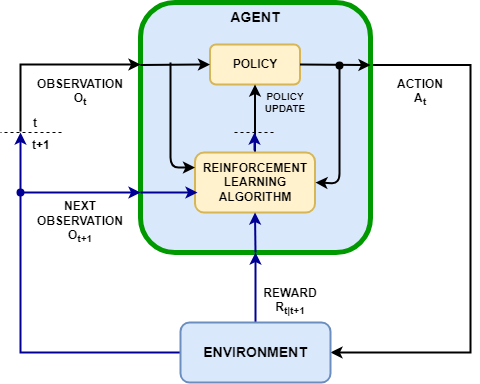
\includegraphics[width=.42\textwidth]{images/rl_scheme.png}
  \caption{RL Agent Scheme}
  {Source: Mathworks\footnotemark} \label{fig:rl_scheme}
\end{figure}
\footnotetext{\url{https://it.mathworks.com/help/reinforcement-learning/ug/create-agents-for-reinforcement-learning.html}}

% \begin{tikzpicture}
%   % Styles
%   \tikzstyle{block}
%   = [rectangle, draw, fill=blue!10, text width=9em, text centered, rounded corners,
%   minimum height=2.5em]
%   \tikzstyle{policy}
%   = [rectangle, draw, fill=yellow!30, text width=9em, text centered, rounded
%   corners, minimum height=2.5em]
%   \tikzstyle{arrow}
%   = [thick, ->, >=stealth]

%   % Agent boundary
%   \draw[thick, rounded corners, fill=blue!5] (-3.5, 2.8) rectangle (3.5, -1.2);
%   \node at (0, 3.1) {\textbf{AGENT}};

%   % Inside the agent: Policy and RL Algorithm
%   \node (policy) [policy] at (0,2) {POLICY};
%   \node (rl)
%     [policy, below=2em of policy]
%     {REINFORCEMENT \\ LEARNING \\ ALGORITHM};

%   % Environment block (positioned below the agent)
%   \node (env) [block, below=6em of rl] {ENVIRONMENT};

%   % Labels for data flow
%   \node[left=4em of policy] (obs) {OBSERVATION };
%   \node[right=4em of policy] (act) {ACTION};
%   \node[below=4em of obs] (next_obs) {NEXT OBSERVATION};
%   \node[above=2em of env] (reward) {REWARD};

%   % Arrows between elements
%   \draw[arrow] (env) -- (reward);
%   \draw[arrow] (env) -| (obs);
%   \draw[arrow] (policy) -- (act);
%   \draw[arrow] (act) |- (env);
%   \draw[arrow] (obs) -- (policy);
%   \draw[arrow] (next_obs) |- (rl);
%   \draw[arrow] (reward) -- (rl);
%   \draw[arrow] (rl) -- (policy) node[midway, right] {POLICY UPDATE};
% \end{tikzpicture}

% \begin{wrapfigure}
%   [17]{l}{.25\textwidth}
%   \centering
%   \def\stackalignment{l}\stackunder{ 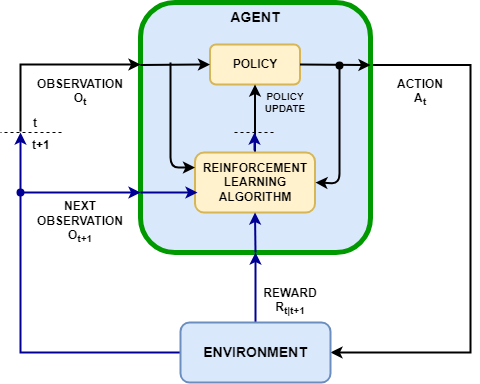
\includegraphics[width=\linewidth]{images/rl_scheme.png} } %
%   {\scriptsize \parbox[t]{\linewidth}{Source: \href{ https://it.mathworks.com/help/reinforcement-learning/ug/create-agents-for-reinforcement-learning.html}{Mathworks}}}
%   \caption{RL Agent Scheme}
%   \label{fig:rl_scheme}
% \end{wrapfigure}
When considering a logistics problem, reinforcement learning naturally comes to
mind. This is because defining a reward function is relatively straightforward—it
could be measured in terms of packages delivered per minute, per step, or a similar
metric. Additionally, the entire process can be simulated in a virtual environment,
allowing multiple parallel simulations to accelerate the agent's learning
process. As illustrated in Figure \ref{fig:rl_scheme}, the structure of the
Reinforcement Learning framework closely resembles the agent-based model
depicted in Figure \ref{fig:agent_scheme}. In both cases, the agent interacts
with its environment, receives feedback in the form of rewards, and continuously
refines its policy to optimize future performance.

Reinforcement Learning works by defining:
\begin{itemize}
  \item \textbf{Environment}: the world in which the agent operates

  \item \textbf{Agent}: the decision-maker that interacts with the environment

  \item \textbf{Actions}: the possible moves the agent can make

  \item \textbf{Rewards}: the feedback the agent receives for its actions

  \item \textbf{Policy}: the strategy the agent uses to select Actions
\end{itemize}

However, RL has its own set of challenges. The most common one is the
convergence to a local minimum in the reward function. This means that the agent
might learn a suboptimal strategy that is not the best one. Moreover, RL is not explainable,
meaning that we can't understand why the agent took a specific action in a
specific situation. This is a big problem in real-world applications, where we
need to understand the decision-making process to ensure safety and reliability.

Another issue with RL is the cost of training. Since the agent learns through trial
and error, it needs to perform a large number of actions to explore the
environment and learn the best strategy. This can be computationally expensive and
time-consuming, especially for complex problems with many variables and states. Moreover,
once the agent is trained, its adaptability to new environments or situations is
limited, as it is optimized for a specific reward function and environment
configuration.

\begin{quotation}
  An example of a problem similar to the one presented in this thesis, solved
  using Reinforcement Learning, can be found in the paper ``DeliverAI: a
  distributed path-sharing network based solution for the last mile food
  delivery problem" by Ashman et al.
\end{quotation}
\subsection{Planning in LLM}

\subsubsection{LLM Agents}
Agenti LLM (es. o1 di OpenAI): introduzione a temi emergenti come il Chain of Thought,
sottolineando come viene eseguito il reasoning e cosa differisce dal mio
approccio